\documentclass[runningheads]{llncs}
\usepackage[T1]{fontenc}

\usepackage{tikz}
\usepackage{listings}
\usetikzlibrary{patterns}

% Definizione dei colori per la sintassi
\definecolor{everforestBg}{HTML}{fffbef}
\definecolor{everforestFg}{HTML}{5c6a72}
\definecolor{everforestRed}{HTML}{f85552}
\definecolor{everforestGreen}{HTML}{8da101}
\definecolor{everforestYellow}{HTML}{dfa000}
\definecolor{everforestBlue}{HTML}{3a94c5}
\definecolor{everforestPurple}{HTML}{df69ba}
\definecolor{everforestAqua}{HTML}{35a77c}
\definecolor{everforestOrange}{HTML}{f57d26}
\definecolor{everforestGray}{HTML}{939f91}

\lstdefinelanguage{AgentSpeak}{
  keywords={
    beliefs, goals, plans, initial_beliefs, initial_goals,
    +, -, !, ?, <-, :, .send, .print, .wait, .my_name, 
    true, false, not, &, |, if, else, for, while
  },
  sensitive=true,
  comment=[l]{//},
  morecomment=[s]{/*}{*/},
  morestring=[b]",
  morestring=[b]',
}

%\lstset{
  %language=AgentSpeak,
  %basicstyle=\ttfamily\small\color{everforestFg},
  %keywordstyle=\color{everforestBlue}\bfseries,
  %commentstyle=\color{everforestGray}\itshape,
  %stringstyle=\color{everforestGreen},
  %numbers=none,
  %%frame=single,
  %%framesep=5pt,
  %breaklines=true,
  %breakatwhitespace=true,
  %showstringspaces=false,
  %%backgroundcolor=\color{everforestBg},
  %rulecolor=\color{everforestFg},
  %%frameround=tttt,
%}

\lstset{
    keywordstyle=\color{blue}\bfseries,
    keywordstyle=[2]\color{teal},
    keywordstyle=[3]\color{red},
    commentstyle=\color{gray}\itshape,
    stringstyle=\color{orange},
    basicstyle=\ttfamily,
    backgroundcolor=\color{white},
    rulecolor=\color{black},
    tabsize=2,
    captionpos=b,
    breaklines=true,
    breakatwhitespace=false,
    showspaces=false,
    showstringspaces=false,
    showtabs=false
}

\title{Towards a Continous Cleaning Robot}
\author{Andrea Gatti\orcidID{0009-0003-0992-4058}}
\institute{University of Genoa}

\begin{document}
	\maketitle

	\begin{abstract}
		The abstract should briefly summarize the contents of the paper in 150--250 words.

		\keywords{First keyword  \and Second keyword \and Another keyword.}
	\end{abstract}

	\section{Introduction}
	\label{sec:introduction}
The cleaning robot is a landmark case study in the world of multi-agent systems, allowing us to think about spatiality with a precise and well-defined goal: to remove all dirt.
The classic example involves a grid environment of which some cells are dirty, and an agent located on it that must find and clean all the dirty cells knowing only how to take a step in one of the four directions and remove the dirt.
With the rapid evolution of game engines, however, the "step-by-step" approach seems to be becoming limiting: we no longer need to think this way; we can abstract more.

In this paper, we propose a cleaning robot that explores space by reasoning about the continuum and leaving the precise management of motion to the environment.

	\section{Related Work}
	\input{sections/related_work.tex}

	\section{Design and Implementation}
	\label{sec:design_and_implementation}
The framework uses JaCaMo for the multi-agent system and Godot for the environment, connected using the WebSocket protocol.

\subsection{Robot Actions}
The agent is able to perform some simple actions: rotate, move, stop and clean.
\begin{figure}
    \centering
    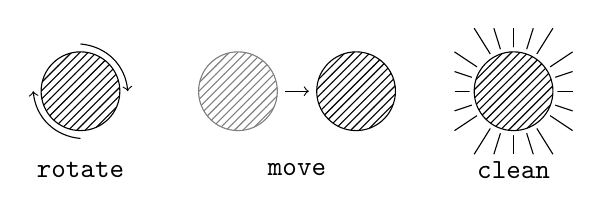
\begin{tikzpicture}
        \draw[pattern=north east lines] (0, 0) circle (0.5cm);
        \draw [->] (0, 0.6) to [bend left=40] (0.6, 0); 
        \draw [->] (0, -0.6) to [bend left=40] (-0.6, 0); 
        \draw (0, -1) node{\texttt{rotate}};

        \draw[black!50!white, pattern=north east lines, pattern color = black!50!white] (2, 0) circle (0.5cm);
        \draw[->] (2.6, 0) -- (2.9, 0);
        \draw[pattern=north east lines] (3.5, 0) circle (0.5cm);
        \draw (2.75, -1) node{\texttt{move}};

        \foreach \x in {5, 5.25, ..., 6}{
            \draw (\x, -0.8) -- (5.5, 0);
            \draw (\x, 0.8) -- (5.5, 0);
        }
        \foreach \y in {-0.5, -0.25, ..., 0.5}{
            \draw (4.75, \y) -- (5.5, 0);
            \draw (6.25, \y) -- (5.5, 0);
        }
        \draw[fill=white, white] (5.5, 0) circle (0.55cm);
        \draw[pattern=north east lines] (5.5, 0) circle (0.5cm);
        \draw (5.5, -1) node{\texttt{clean}};
    \end{tikzpicture}
\end{figure}
These actions are implemented as simple plans in the agent body.
Here we present the motion action as example.
\begin{lstlisting}[language=AgentSpeak]
+!move
    :   true
    <-  .print("Moving robot");
        move.
\end{lstlisting}
In this case the action is to move and the agent calls the \lstinline{move} artifact method.
\begin{lstlisting}[language=java]
@OPERATION
public void move(){
    JSONObject json = new JSONObject();
    json.put("type", "move");
    json.put("status", "start");
    send(json);
}
\end{lstlisting}

\subsection{Logic Exploration}

\begin{figure}
    \centering
    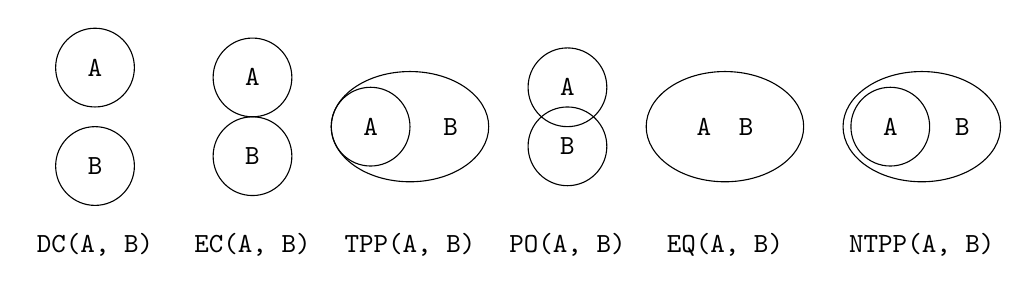
\begin{tikzpicture}
    \draw (0, 1.25) circle (0.5cm) node{\texttt{A}};
    \draw (0, 0) circle (0.5cm) node{\texttt{B}};
    \draw (0, -1) node{\texttt{DC(A, B)}};

    \draw (2, 1.125) circle (0.5cm) node{\texttt{A}};
    \draw (2, 0.125) circle (0.5cm) node{\texttt{B}};
    \draw (2, -1) node{\texttt{EC(A, B)}};

    \draw (3.5, 0.5) circle (0.5cm) node{\texttt{A}};
    \draw (4, 0.5) ellipse (1cm and 0.7cm) node[right=0.3cm]{\texttt{B}};
    \draw (4, -1) node{\texttt{TPP(A, B)}};

    \draw (6, 1) circle (0.5cm) node{\texttt{A}};
    \draw (6, 0.25) circle (0.5cm) node{\texttt{B}};
    \draw (6, -1) node{\texttt{PO(A, B)}};

    \draw (8, 0.5) ellipse (1cm and 0.7cm) node{\texttt{A} \ \ \texttt{B}};
    \draw (8, -1) node{\texttt{EQ(A, B)}};

    \draw (10.1, 0.5) circle (0.5cm) node{\texttt{A}};
    \draw (10.5, 0.5) ellipse (1cm and 0.7cm) node[right=0.3cm]{\texttt{B}};
    \draw (10.5, -1) node{\texttt{NTPP(A, B)}};

\end{tikzpicture}
    \label{fig:relations}
    \caption{Relations between regions}
\end{figure}

\begin{figure}[ht]
    \centering
        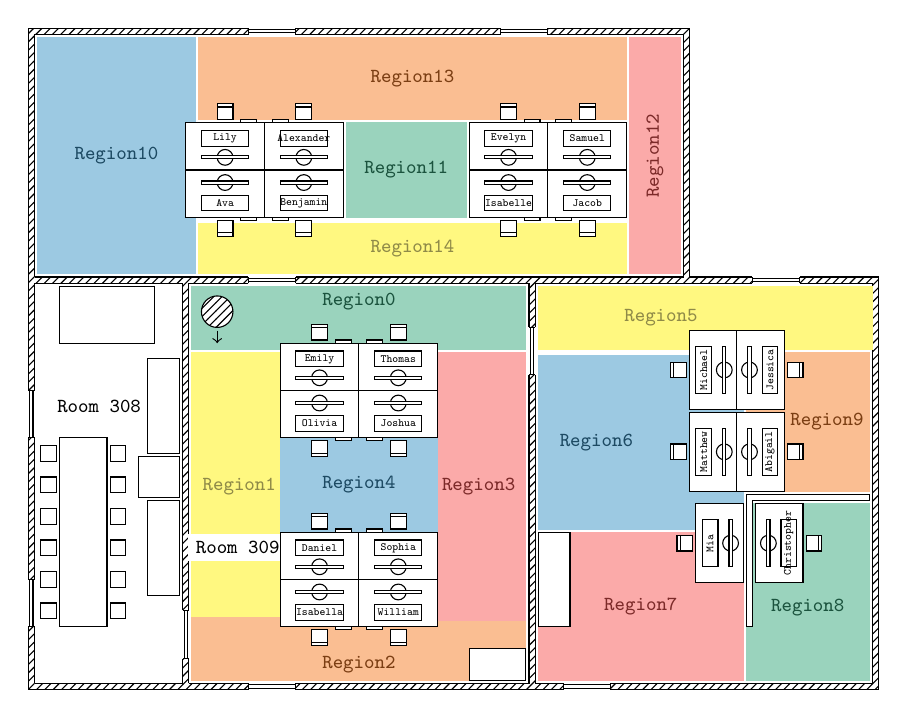
\begin{tikzpicture}[scale=0.4, every node/.style={scale=0.8}]
        % Area
        \draw[pattern=north east lines] (0,0) -- (0, 21) -- (21, 21) -- (21, 13.1) -- (27, 13.1) -- (27, 0) -- (0, 0);
        % Rooms
        \draw[fill=white] (0.2, 0.2) -- (0.2, 12.9) -- (4.9, 12.9) -- (4.9, 0.2) -- (0.2, 0.2);
        \draw (2.25, 9) node{\small\tt Room 308};
        \draw[fill=white] (5.1, 0.2) -- (5.1, 12.9) -- (15.9, 12.9) -- (15.9, 0.2) -- (5.1, 0.2);
        \draw[fill=white] (16.1, 0.2) -- (16.1, 12.9) -- (26.8, 12.9) -- (26.8, 0.2) -- (16.1, 0.2);
        \draw (18, 6.5) node{\small\tt Room 310};
        \draw[fill=white] (0.2, 13.1) -- (0.2, 20.8) -- (20.8, 20.8) -- (20.8, 13.1) -- (0.2, 13.1);
        \draw (4, 17) node{\small\tt Room 314};

        \draw[fill=everforestAqua!50!white, everforestAqua!50!white] (5.2, 10.8) rectangle node[above, everforestAqua!50!black]{\small\tt Region0} ++ (10.6, 2);
        \draw[fill=yellow!50!white, yellow!50!white] (5.2, 2.2) rectangle node[yellow!50!black]{\small\tt Region1} ++ (3, 8.5);
        \draw[fill=everforestOrange!50!white, everforestOrange!50!white] (5.2, 0.3) rectangle node[below, everforestOrange!50!black]{\small\tt Region2} ++ (10.6, 2);
        \draw[fill=everforestRed!50!white, everforestRed!50!white] (12.8, 2.2) rectangle node[everforestRed!50!black]{\small\tt Region3} ++ (3, 8.5);
        \draw[fill=everforestBlue!50!white, everforestBlue!50!white] (8, 5) rectangle node[everforestBlue!50!black]{\small\tt Region4} ++ (5, 3);

        \draw[fill=yellow!50!white, yellow!50!white] (16.2, 10.8) rectangle node[left, yellow!50!black]{\small\tt Region5} ++ (10.6, 2);
        \draw[fill=everforestBlue!50!white, everforestBlue!50!white] (16.2, 5.1) rectangle node[left, everforestBlue!50!black]{\small\tt Region6} ++ (6.5, 5.5);
        \draw[fill=everforestRed!50!white, everforestRed!50!white] (16.2, 0.3) rectangle node[everforestRed!50!black]{\small\tt Region7} ++ (6.5, 4.7);
        \draw[fill=everforestAqua!50!white, everforestAqua!50!white] (22.8, 0.3) rectangle node[below, everforestAqua!50!black]{\small\tt Region8} ++ (3.9, 5.6);
        \draw[fill=everforestOrange!50!white, everforestOrange!50!white] (22.8, 6.3) rectangle node[right=-0.4cm, everforestOrange!50!black]{\small\tt Region9} ++ (3.9, 4.4);

        \draw[fill=everforestBlue!50!white, everforestBlue!50!white] (0.3, 13.2) rectangle node[everforestBlue!50!black]{\small\tt Region10} ++ (5, 7.5);
        \draw[fill=everforestAqua!50!white, everforestAqua!50!white] (10.1, 15) rectangle node[everforestAqua!50!black]{\small\tt Region11} ++ (3.8, 3);
        \draw[fill=everforestRed!50!white, everforestRed!50!white] (19.1, 13.2) rectangle node[rotate=90,everforestRed!50!black]{\small\tt Region12} ++ (1.6, 7.5);
        \draw[fill=everforestOrange!50!white, everforestOrange!50!white] (5.4, 18.1) rectangle node[everforestOrange!50!black]{\small\tt Region13} ++ (13.6, 2.6);
        \draw[fill=yellow!50!white, yellow!50!white] (5.4, 13.2) rectangle node[yellow!50!black]{\small\tt Region14} ++ (13.6, 1.6);

        \draw (6.65, 4.5) node[fill=white]{\small\tt Room 309};

        % Door 309 Bottom
        \draw[fill=white, white] (7, 0) rectangle ++ (1.5, 0.2);
        \draw (7, 0) -- (7, 0.2) (8.5, 0) -- (8.5, 0.2);
        \draw (7, 0.05) rectangle ++ (1.5, 0.1);

        % Door 310 Bottom
        \draw[fill=white, white] (17, 0) rectangle ++ (1.5, 0.2);
        \draw (17, 0) -- (17, 0.2) (18.5, 0) -- (18.5, 0.2);
        \draw (17, 0.05) rectangle ++ (1.5, 0.1);

        % Door 309 Top
        \draw[fill=white, white] (7, 12.9) rectangle ++ (1.5, 0.2);
        \draw (7, 12.9) -- (7, 13.1) (8.5, 12.9) -- (8.5, 13.1);
        \draw (7, 12.95) rectangle ++ (1.5, 0.1);

        % Door 310 Top
        \draw[fill=white, white] (23, 12.9) rectangle ++ (1.5, 0.2);
        \draw (23, 12.9) -- (23, 13.1) (24.5, 12.9) -- (24.5, 13.1);
        \draw (23, 12.95) rectangle ++ (1.5, 0.1);

        % Door 314 Left
        \draw[fill=white, white] (7, 20.8) rectangle ++ (1.5, 0.2);
        \draw (7, 20.8) -- (7, 21) (8.5, 20.8) -- (8.5, 21);
        \draw (7, 20.85) rectangle ++ (1.5, 0.1);

        % Door 314 Right
        \draw[fill=white, white] (15, 20.8) rectangle ++ (1.5, 0.2);
        \draw (15, 20.8) -- (15, 21) (16.5, 20.8) -- (16.5, 21);
        \draw (15, 20.85) rectangle ++ (1.5, 0.1);

        % Door 308 Bottom
        \draw[fill=white, white] (0, 2) rectangle ++ (0.2, 1.5);
        \draw (0, 2) -- (0.2, 2) (0, 3.5) -- (0.2, 3.5);
        \draw (0.05, 2) rectangle ++ (0.1, 1.5);

        % Door 308-309
        \draw[fill=white, white] (4.9, 1) rectangle ++ (0.2, 1.5);
        \draw (4.9, 1) -- (5.1, 1) (4.9, 2.5) -- (5.1, 2.5);
        \draw (4.95, 1) rectangle ++ (0.1, 1.5);

        % Door 308 Top
        \draw[fill=white, white] (0, 8) rectangle ++ (0.2, 1.5);
        \draw (0, 8) -- (0.2, 8) (0, 9.5) -- (0.2, 9.5);
        \draw (0.05, 8) rectangle ++ (0.1, 1.5);

        % Door 309-310
        \draw[fill=white, white] (15.9, 10) rectangle ++ (0.2, 1.5);
        \draw (15.9, 10) -- (16.1, 10) (15.9, 11.5) -- (16.1, 11.5);
        \draw (15.95, 10) rectangle ++ (0.1, 1.5);

        % Desk Bottom Down Left
        \draw[fill=white] (8, 2) rectangle ++ (2.5, 1.5);
        % Chair
        \draw[fill=white] (9, 1.4) rectangle ++ (0.5, 0.5);
        \draw[fill=white] (9, 1.4) rectangle ++ (0.5, 0.1);
        \draw[fill=white] (9.75, 1.9) rectangle ++ (0.5, 0.1);
        % Computer
        \draw (9.25, 3.1) circle (0.25cm);
        \draw[fill=white] (8.5, 3.05) rectangle ++ (1.5, 0.1);
        \draw (8.5, 2.2) rectangle node{\tiny\tt Isabella} ++ (1.5, 0.5);

        % Desk Bottom Down Right
        \draw[fill=white] (10.5, 2) rectangle ++ (2.5, 1.5);
        % Chair
        \draw[fill=white] (11.5, 1.4) rectangle ++ (0.5, 0.5);
        \draw[fill=white] (11.5, 1.4) rectangle ++ (0.5, 0.1);
        \draw[fill=white] (10.75, 1.9) rectangle ++ (0.5, 0.1);
        % Computer
        \draw (11.75, 3.1) circle (0.25cm);
        \draw[fill=white] (11, 3.05) rectangle ++ (1.5, 0.1);
        \draw (11, 2.2) rectangle node{\tiny\tt William}++ (1.5, 0.5);

        % Desk Bottom Up Left
        \draw[fill=white] (8, 3.5) rectangle ++ (2.5, 1.5);
        % Chair
        \draw[fill=white] (9, 5.1) rectangle ++ (0.5, 0.5);
        \draw[fill=white] (9, 5.5) rectangle ++ (0.5, 0.1);
        \draw[fill=white] (9.75, 5) rectangle ++ (0.5, 0.1);
        % Computer
        \draw (9.25, 3.9) circle (0.25cm);
        \draw[fill=white] (8.5, 3.85) rectangle ++ (1.5, 0.1);
        \draw (8.5, 4.25) rectangle node{\tiny\tt Daniel} ++ (1.5, 0.5);

        % Desk Bottom Up Right
        \draw[fill=white] (10.5, 3.5) rectangle ++ (2.5, 1.5);
        % Chair
        \draw[fill=white] (11.5, 5.1) rectangle ++ (0.5, 0.5);
        \draw[fill=white] (11.5, 5.5) rectangle ++ (0.5, 0.1);
        \draw[fill=white] (10.75, 5) rectangle ++ (0.5, 0.1);
        % Computer
        \draw (11.75, 3.9) circle (0.25cm);
        \draw[fill=white] (11, 3.85) rectangle ++ (1.5, 0.1);
        \draw (11, 4.25) rectangle node{\tiny\tt Sophia} ++ (1.5, 0.5);

        \draw[fill=white] (8, 8) rectangle ++ (2.5, 1.5);
        \draw[fill=white] (9, 7.4) rectangle ++ (0.5, 0.5);
        \draw[fill=white] (9, 7.4) rectangle ++ (0.5, 0.1);
        \draw[fill=white] (9.75, 7.9) rectangle ++ (0.5, 0.1);
        % Computer
        \draw (9.25, 9.1) circle (0.25cm);
        \draw[fill=white] (8.5, 9.05) rectangle ++ (1.5, 0.1);
        \draw (8.5, 8.2) rectangle node{\tiny\tt Olivia} ++ (1.5, 0.5);

        \draw[fill=white] (10.5, 8) rectangle ++ (2.5, 1.5);
        \draw[fill=white] (11.5, 7.4) rectangle ++ (0.5, 0.5);
        \draw[fill=white] (11.5, 7.4) rectangle ++ (0.5, 0.1);
        \draw[fill=white] (10.75, 7.9) rectangle ++ (0.5, 0.1);

        \draw[fill=white] (8, 9.5) rectangle ++ (2.5, 1.5);
        \draw[fill=white] (9, 11.1) rectangle ++ (0.5, 0.5);
        \draw[fill=white] (9, 11.5) rectangle ++ (0.5, 0.1);
        \draw[fill=white] (9.75, 11) rectangle ++ (0.5, 0.1);
        % Computer
        \draw (9.25, 9.9) circle (0.25cm);
        \draw[fill=white] (8.5, 9.85) rectangle ++ (1.5, 0.1);
        \draw (8.5, 10.25) rectangle node{\tiny\tt Emily} ++ (1.5, 0.5);

        \draw[fill=white] (10.5, 9.5) rectangle ++ (2.5, 1.5);
        \draw[fill=white] (11.5, 11.1) rectangle ++ (0.5, 0.5);
        \draw[fill=white] (11.5, 11.5) rectangle ++ (0.5, 0.1);
        \draw[fill=white] (10.75, 11) rectangle ++ (0.5, 0.1);
        % Computer
        \draw (11.75, 9.1) circle (0.25cm);
        \draw[fill=white] (11, 9.05) rectangle ++ (1.5, 0.1);
        \draw (11, 8.2) rectangle node{\tiny\tt Joshua} ++ (1.5, 0.5);
        % Computer
        \draw (11.75, 9.9) circle (0.25cm);
        \draw[fill=white] (11, 9.85) rectangle ++ (1.5, 0.1);
        \draw (11, 10.25) rectangle node{\tiny\tt Thomas} ++ (1.5, 0.5);

        \draw[fill=white] (14, 0.3) rectangle ++ (1.8, 1);

        \draw (1, 2) rectangle ++ (1.5, 6);
        \foreach \x in {2.25, 3.25, ..., 7.25} {
            \draw (2.6, \x) rectangle ++ (0.5, 0.5); 
            \draw (0.4, \x) rectangle ++ (0.5, 0.5); 
        }
        
        \draw (3.8, 3) rectangle ++ (1, 3);
        \draw (3.5, 6.1) rectangle ++ (1.3, 1.3);
        \draw (3.8, 7.5) rectangle ++ (1, 3);
        \draw (1, 11) rectangle ++ (3, 1.8);

        \draw[fill=white] (23, 2) -- (23, 6) -- (26.7, 6) -- (26.7, 6.2) -- (22.8, 6.2) -- (22.8, 2) -- (23, 2);

        \draw[fill=white] (21, 8.9) rectangle ++ (1.5, 2.5);
        \draw[fill=white] (20.4, 9.9) rectangle ++ (0.5, 0.5);
        \draw[fill=white] (20.4, 9.9) rectangle ++ (0.1, 0.5);
        \draw[fill=white] (22.1, 10.15) circle (0.25cm);
        \draw[fill=white] (22.05, 9.4) rectangle ++ (0.1, 1.5);
        \draw (21.2, 9.4) rectangle node[rotate=90]{\tiny\tt Michael} ++ (0.5, 1.5);

        \draw[fill=white] (22.5, 8.9) rectangle ++ (1.5, 2.5);
        \draw[fill=white] (24.1, 9.9) rectangle ++ (0.5, 0.5);
        \draw[fill=white] (24.5, 9.9) rectangle ++ (0.1, 0.5);
        \draw[fill=white] (22.9, 10.15) circle (0.25cm);
        \draw[fill=white] (22.85, 9.4) rectangle ++ (0.1, 1.5);
        \draw (23.3, 9.4) rectangle node[rotate=90]{\tiny\tt Jessica} ++ (0.5, 1.5);

        \draw[fill=white] (21, 6.3) rectangle ++ (1.5, 2.5);
        \draw[fill=white] (20.4, 7.3) rectangle ++ (0.5, 0.5);
        \draw[fill=white] (20.4, 7.3) rectangle ++ (0.1, 0.5);
        \draw (22.1, 7.55) circle (0.25cm);
        \draw[fill=white] (22.05, 6.8) rectangle ++ (0.1, 1.5);
        \draw (21.2, 6.8) rectangle node[rotate=90]{\tiny\tt Matthew} ++ (0.5, 1.5);

        \draw[fill=white] (22.5, 6.3) rectangle ++ (1.5, 2.5);
        \draw[fill=white] (24.1, 7.3) rectangle ++ (0.5, 0.5);
        \draw[fill=white] (24.5, 7.3) rectangle ++ (0.1, 0.5);
        \draw (22.9, 7.55) circle (0.25cm);
        \draw[fill=white] (22.85, 6.8) rectangle ++ (0.1, 1.5);
        \draw (23.3, 6.8) rectangle node[rotate=90]{\tiny\tt Abigail} ++ (0.5, 1.5);

        \draw[fill=white] (21.2, 3.4) rectangle ++ (1.5, 2.5);
        \draw[fill=white] (20.6, 4.4) rectangle ++ (0.5, 0.5);
        \draw[fill=white] (20.6, 4.4) rectangle ++ (0.1, 0.5);
        \draw (22.3, 4.65) circle (0.25cm);
        \draw[fill=white] (22.25, 3.9) rectangle ++ (0.1, 1.5);
        \draw (21.4, 3.9) rectangle node[rotate=90]{\tiny\tt Mia} ++ (0.5, 1.5);

        \draw[fill=white] (23.1, 3.4) rectangle ++ (1.5, 2.5);
        \draw[fill=white] (24.7, 4.4) rectangle ++ (0.5, 0.5);
        \draw[fill=white] (25.1, 4.4) rectangle ++ (0.1, 0.5);
        \draw (23.5, 4.65) circle (0.25cm);
        \draw[fill=white] (23.45, 3.9) rectangle ++ (0.1, 1.5);
        \draw (23.9, 3.9) rectangle node[rotate=90]{\tiny\tt Christopher} ++ (0.5, 1.5);

        % Desk Bottom Down Left
        \draw[fill=white] (5, 15) rectangle ++ (2.5, 1.5);
        % Chair
        \draw[fill=white] (6, 14.4) rectangle ++ (0.5, 0.5);
        \draw[fill=white] (6, 14.4) rectangle ++ (0.5, 0.1);
        \draw[fill=white] (6.75, 14.9) rectangle ++ (0.5, 0.1);
        % Computer
        \draw (6.25, 16.1) circle (0.25cm);
        \draw[fill=white] (5.5, 16.05) rectangle ++ (1.5, 0.1);
        \draw (5.5, 15.2) rectangle node{\tiny\tt Ava} ++ (1.5, 0.5);

        % Desk Bottom Down Right
        \draw[fill=white] (7.5, 15) rectangle ++ (2.5, 1.5);
        % Chair
        \draw[fill=white] (8.5, 14.4) rectangle ++ (0.5, 0.5);
        \draw[fill=white] (8.5, 14.4) rectangle ++ (0.5, 0.1);
        \draw[fill=white] (7.75, 14.9) rectangle ++ (0.5, 0.1);
        % Computer
        \draw (8.75, 16.1) circle (0.25cm);
        \draw[fill=white] (8, 16.05) rectangle ++ (1.5, 0.1);
        \draw (8, 15.2) rectangle node{\tiny\tt Benjamin} ++ (1.5, 0.5);

        % Desk Bottom Up Left
        \draw[fill=white] (5, 16.5) rectangle ++ (2.5, 1.5);
        % Chair
        \draw[fill=white] (6, 18.1) rectangle ++ (0.5, 0.5);
        \draw[fill=white] (6, 18.5) rectangle ++ (0.5, 0.1);
        \draw[fill=white] (6.75, 18) rectangle ++ (0.5, 0.1);
        % Computer
        \draw (6.25, 16.9) circle (0.25cm);
        \draw[fill=white] (5.5, 16.85) rectangle ++ (1.5, 0.1);
        \draw (5.5, 17.25) rectangle node{\tiny\tt Lily} ++ (1.5, 0.5);

        % Desk Bottom Up Right
        \draw[fill=white] (7.5, 16.5) rectangle ++ (2.5, 1.5);
        \draw[fill=white] (8.5, 18.1) rectangle ++ (0.5, 0.5);
        \draw[fill=white] (8.5, 18.5) rectangle ++ (0.5, 0.1);
        \draw[fill=white] (7.75, 18) rectangle ++ (0.5, 0.1);
        % Computer
        \draw (8.75, 16.9) circle (0.25cm);
        \draw[fill=white] (8, 16.85) rectangle ++ (1.5, 0.1);
        \draw (8, 17.25) rectangle node{\tiny\tt Alexander} ++ (1.5, 0.5);

        % Desk Bottom Down Left
        \draw[fill=white] (14, 15) rectangle ++ (2.5, 1.5);
        \draw[fill=white] (15, 14.4) rectangle ++ (0.5, 0.5);
        \draw[fill=white] (15, 14.4) rectangle ++ (0.5, 0.1);
        \draw[fill=white] (15.75, 14.9) rectangle ++ (0.5, 0.1);
        % Computer
        \draw (15.25, 16.1) circle (0.25cm);
        \draw[fill=white] (14.5, 16.05) rectangle ++ (1.5, 0.1);
        \draw (14.5, 15.2) rectangle node{\tiny\tt Isabelle} ++ (1.5, 0.5);

        % Desk Bottom Down Right
        \draw[fill=white] (16.5, 15) rectangle ++ (2.5, 1.5);
        % Chair
        \draw[fill=white] (17.5, 14.4) rectangle ++ (0.5, 0.5);
        \draw[fill=white] (17.5, 14.4) rectangle ++ (0.5, 0.1);
        \draw[fill=white] (16.75, 14.9) rectangle ++ (0.5, 0.1);
        % Computer
        \draw (17.75, 16.1) circle (0.25cm);
        \draw[fill=white] (17, 16.05) rectangle ++ (1.5, 0.1);
        \draw (17, 15.2) rectangle node{\tiny\tt Jacob} ++ (1.5, 0.5);

        % Desk Bottom Up Left
        \draw[fill=white] (14, 16.5) rectangle ++ (2.5, 1.5);
        \draw[fill=white] (15, 18.1) rectangle ++ (0.5, 0.5);
        \draw[fill=white] (15, 18.5) rectangle ++ (0.5, 0.1);
        \draw[fill=white] (15.75, 18) rectangle ++ (0.5, 0.1);
        % Computer
        \draw (15.25, 16.9) circle (0.25cm);
        \draw[fill=white] (14.5, 16.85) rectangle ++ (1.5, 0.1);
        \draw (14.5, 17.25) rectangle node{\tiny\tt Evelyn} ++ (1.5, 0.5);

        % Desk Bottom Up Right
        \draw[fill=white] (16.5, 16.5) rectangle ++ (2.5, 1.5);
        \draw[fill=white] (17.5, 18.1) rectangle ++ (0.5, 0.5);
        \draw[fill=white] (17.5, 18.5) rectangle ++ (0.5, 0.1);
        \draw[fill=white] (16.75, 18) rectangle ++ (0.5, 0.1);
        % Computer
        \draw (17.75, 16.9) circle (0.25cm);
        \draw[fill=white] (17, 16.85) rectangle ++ (1.5, 0.1);
        \draw (17, 17.25) rectangle node{\tiny\tt Samuel} ++ (1.5, 0.5);

        \draw[fill=white] (16.2, 2) rectangle ++ (1, 3);

        \draw[preaction={fill, white}, black, pattern=north east lines] (6, 12) circle (0.5cm);
        \draw[->] (6, 11.4) -- (6, 11);
    \end{tikzpicture}
    \label{fig:environment}
    \caption{The test environment}
\end{figure}

	\section{Results}
	\label{sec:results}
In this section we briefly present the results obtained.
The agent communicates correctly with the virtual robot and manages to complete its task completely.
It is possible to see the operation of the framework in two videos, \href{https://youtu.be/dQbiNx36fNs}{one} in which the agent simply performs its task and \href{https://youtu.be/iuQfDgS0oUE}{one} in which the debug mode is activated in which we can see the paths calculated by the robot.

\begin{figure}
    \centering
    \includegraphics[width=\textwidth]{sections/imgs/screen.jpeg}
    \caption{The agent in action.}
    \label{fig:screen}
\end{figure}
In the Figure\ref{fig:screen} you can see the framework in action.
On the left is the JaCaMo window in which the agent is implemented while on the right is visible Godot and the robot you want in the room.

In the implementation we were able to completely separate the logical reasoning part from the coordinate management part.
For the time being, however, the agent is still not looking for the best path but simply for a walkable path from one region to another.
The results confirm that the robot in this way has full freedom of rotation by producing non-regular paths and that the ability to find paths in the instrument continuum is enhanced.
The robot's path planning, in addition to the features already listed, also has the ability to adapt to any occlusions dynamically, recalculating the path in case something has moved without having to take it into account logically.

This implementation is easily scalable from both the environment and multi-agent system perspectives.
In fact, the region-based logic model makes it very easy to expand the environment both in width and depth (increasing its accuracy); in fact, we have already demonstrated the operation of subregions by implementing rooms.
The connection between agent and robot implemented end-to-end with a private artifact of the agent and a proven script of the robot also makes the multi-agent system scalable without the need for further major modifications.

	\section{Conclusions}
	We presented a framework in which a BDI agent controls a robot vacuum cleaner with a precise division of responsibilities, giving logical task management to the agent and physical management of movement and cleaning to the robot.
Going through the key theoretical concepts, we showed how the environment must be studied and designed for this kind of approach, then going on to see the actual implementation of all components with JaCaMo and Godot.
The implementation aims not to discretize the robot's movements by forcing them within some predetermined logical actions but by choosing the actions logically, implementing them in the continuum.

The current implementation has many limitations, the two most important being the management of regions on the virtual environment side and the insertion of objects into the logical map.
In Godot, the region should be implemented as an Area3D, looking for the nearest location without having to reach the center or a specific point.
Agent side, the map should also contain objects and objects should be considered, thinking of a scenario where they are most meaningful.

Future work will therefore go in these directions.
In addition to this, an exploratory version of the framework will be implemented in which the agent faces the challenge of cleaning without knowing the map and without knowing where the dirty areas are.
The real challenge in this version will be to figure out how to subdivide the walkable regions, what are the criteria that make a region stand on its own or not.

\end{document}